\chapter{基于雷尼散度的有辅助信息的随机块模型研究}
\label{chap:sbmsi}
\section{本章引言}
在本章中,我们首先介绍有辅助信息的随机块模型
的定义。
我们在前人研究的基础上,给出两社团情形下的精确恢复条件。
在精确恢复条件被保证的前提下,
我们将利用雷尼散度这一度量进一步研究
具有不同稀疏程度的模型的误差衰减率。
除此之外,我们将证明通过求解某半正定规划问题,可实现精确
恢复的要求,而该等价的优化问题可通过交替方向乘子法(ADMM)进行求解。

本章内容的具体安排如下:
在\ref{sec:sbmsi_exact_recovery_condition}节,我们给出了
带有辅助信息的随机块模型的精确恢复条件;
在\ref{sec:sbmsi_error_decay_rate}节,我们研究了算法的最优误差衰减速率,
在\ref{sec:sdp_exact}节,我们给出了一个能实现精确恢复的SDP算法,并通过实验
验证了其精确恢复效果。
第\ref{sec:summary_sbmsi}节对全章进行了总结。

\section{精确恢复条件}\label{sec:sbmsi_exact_recovery_condition}
\newacronym{acr:sbmsi}{SBMSI}{Stochastic Block Model with side information}
带有辅助信息的随机块模型(\gls{acr:sbmsi})
是\ref{sec:sbm}节介绍的
SSBM 模型的推广。为方便讨论又不失一般性,
这里我们在2个社团的随机块模型的
基础上引入辅助信息。
由定义\ref{def:SSBM},当$k=2$时,
节点标签$X$满足$X_i \in \{\pm 1\}$
且 $\sum_{i=1}^n X_i = 0$。
除了图中边的集合
$\{Z_{i,j}\}_{1\le i<j\le n}$
和节点标签 $X$ 外,
第 $i$  个节点 ($1\leq i \leq n$) 
还含有 $m=\lceil \gamma \log n \rceil $ 个相关的数据样本 
$\{Y^{i}_j\}_{1\leq j \leq m}$。
这里,我们要求 $\gamma$ 是一个正整数。
若 $X_i=1$,
这些样本 i.i.d. 采样自分布 $P_0$,
若 $X_i=-1$,则采样自 $P_1$。
这里假设 $P_0, P_1$ 两个分布函数均为定义在字母集$\mathcal{Y}$上的离散分布。
注意到 给定 标签 $X_i$,
对于 $i\in [n]$,数据样本 $\{Y^{i}_j\}_{1\leq j \leq m}$ 与 $\{Z_{i,j}\}_{1\le i<j\le n}$ 独立。
 因此,在标签 $X$ 给定的情况下,
  $(\{Z_{i,j}\}_{1\le i<j\le n},\{Y^i_{j}\}_{1\le i\le n,1\le j\le m})$ 的联合分布为  
\begin{align}\label{eq:lh}
    &P(y=\{y^i_{j}\}_{1\le i\le n,1\le j\le m},z=\{z_{i,j}\}_{1\le i<j\le n}| (x_1,\ldots,x_n)) \nonumber\\
    &= \prod_{1\le i < j\le n}P(z_{i,j}|x_i,x_j)\prod_{i=1}^n \prod_{j=1}^m P(y^i_j|x_i), 
\end{align}
其中$\prod_{1\le i,j\le n}P(z_{i,j}|x_i,x_j)$ 可写成
式\eqref{eq:mle_sibm} 的形式。
对于$P(z_{i,j}|x_i,x_j)$,其具体定义为
\begin{equation*}
    P  (z_{i,j}=1|x_i,x_j) = \begin{cases}
        p & \text{if } x_i = x_j \\
        q & \text{if } x_i\ne x_j
    \end{cases},
\end{equation*}
并且
\begin{equation*}
    P(y^i_j|x_i) = \begin{cases}
        P_0(y^i_j) & x_i = 1 \\
        P_1(y^i_j) & x_i = -1
    \end{cases}
\end{equation*}
 $P(\{y^i_{j}\}_{1\le i\le n,1\le j\le m},\{z_{i,j}\}_{1\le i<j\le n}| x_1,\ldots,x_n)$ 
 的条件分布 依赖于
 $n,m,p, q, P_0$ 和 $P_1$ 这些参数,因此我们把 SBMSI 写成 $\SBMSI(n,m,p,q,P_0,P_1)$ 的形式。
 给定由 $\SBMSI(n,m,p,q,P_0,P_1)$ 生成的边$Z$和数据$Y$, 我们的目标是恢复 出$X$。
 
 在有辅助信息$Y$的条件下,
 我们仍使用能否精确恢复这一指标来衡量
 社团发现算法的准确性。
 与定义\ref{def:SSBMR}类似,
 若存在以$Z,Y$为输入变量的算法 $\hat{X}=\hat{X}(Z,Y)$
 使得当$n$增大时,
 错误概率
 $P_e:=P(\hat{Y} \neq Y)$ 趋向于 $0$,则称
 精确恢复可实现。

 文献\inlinecite{abbe2015community}中的3.2小节指出了一般随机块模型
 的精确恢复条件与多维泊松分布的关系。
在$k=2$的情形,我们要用到2维泊松分布,因此这里对其做一个简单的介绍。
有多种方式可推广一维的泊松分布,这里我们使用的是如下形式的二维泊松分布:

\begin{definition}
    称 $(X,Y)$ 服从参数为 $(\lambda, \mu)$ 的二维泊松分布,
    如果其概率质量函数为:
    \begin{equation}
        P(X=k, Y=j) = \frac{\lambda^k \mu^j}{k! j!}
        e^{-\lambda - \mu}, k,j=0,1,\dots
    \end{equation}
    记为 $(X,Y) \sim \Pois(\lambda, \mu)$。
\end{definition}

有了2维泊松分布的定义式,我们下面给出
SBMSI 模型精确恢复的条件:
\begin{theorem}\label{thm:Pe}
    定义$I_+$ 为联合分布 $\textrm{Pois}(\frac{a}{2},\frac{b}{2})\times \underbrace{P_0 \times \dots \times P_0}_{\gamma}$
    与 $\textrm{Pois}(\frac{b}{2}, \frac{a}{2})\times \underbrace{P_1 \times \dots \times P_1}_{\gamma}$ 
    之间的切尔诺夫信息。    
    对于 $\SBMSI(n,m=\lceil \gamma \log n \rceil, p=a\frac{\log n}{n},q=b\frac{\log n}{n},P_0,P_1)$,
    如果 $I_+>1$,则精确恢复可实现;
    如果 $I_+ < 1$,
    则错误概率 $P_e$ 趋近于 $1$,精确恢复不可实现。
\end{theorem}

定理\ref{thm:Pe}类似于文献 \inlinecite{abbe17sideinfo} 中定理4的结论,
但这里我们允许采样数量 $m$ 为
$\lceil \log n \rceil $ 的整数倍,同时
限制了类别数为2的条件,而 文献 \inlinecite{abbe17sideinfo} 的定理4
中始终取$\gamma=1$。

对于一般的情形,SBMSI 模型精确恢复的 临界值 $I_+$ 并没有
显示表达式,但我们可以从切尔诺夫信息的定义出发得到 $I_+$ 的简化表达式,
该表达式由下述引理\ref{lem:I_plus_expression}给出,
其更容易计算,且在后面定理\ref{thm:sdp}的证明中也会用到。

\begin{lemma}\label{lem:I_plus_expression}
\begin{align}\label{equation:I+}
    I_+ &=\frac{\lambda^* }{2} (a^{1-\lambda^* }b^{\lambda^* } -
    b^{1-\lambda^* }a^{\lambda^* })\log\frac{b}{a}+\frac{a+b}{2}\notag \\
    &-\frac{1}{2}(a^{1-\lambda^*}b^{\lambda^*} +
    b^{1-\lambda^* }a^{\lambda^* })+\gamma D(P_{\lambda^* }||P_0) 
	\end{align}
	其中
	\begin{equation}\label{eq:lambda}
    \lambda^* = \arg\min_{\lambda} \left[a^{1-\lambda}b^{\lambda} +
    b^{1-\lambda}a^{\lambda} + 2\gamma \log
    \left(\sum_{x\in \mathcal{X}}P^{1-\lambda}_0(x) P^{\lambda}_1(x)
    \right)
    \right]
\end{equation}
而 $P_{\lambda}$ 类似式\eqref{eq:P_lambda_x} ,为
\begin{equation}\label{eq:P_lambda_0_1}
    P_{\lambda}(x) = \frac{P_0^{1-\lambda}(x) P_1^{\lambda} (x)}
    {\sum_{x \in \mathcal{X}}P_0^{1-\lambda}(x) P_1^{\lambda} (x)}        
\end{equation}

\end{lemma}


%\section{引理\ref{lem:I_plus_expression} 的证明}
在证明引理
\ref{lem:I_plus_expression}  之前,
我们先列举泊松分布的一个重要的性质。
\begin{lemma}\label{lem:poisson_property}
假设 $P_0 \sim \Pois(c)$, $P_1 \sim \Pois(d)$.
且 $P_{\lambda}$ 由 式\eqref{eq:P_lambda_0_1}
给出。

则我们有
\begin{enumerate}
    \item $P_{\lambda} \sim \Pois(c^{1-\lambda} d^{\lambda})$
    \item $D(P_{\lambda}||P_0) = 
    \lambda c^{1-\lambda}d^{\lambda}\log(\frac{d}{c}) + c-c^{1-\lambda}d^{\lambda}$
    \item $D(P_{\lambda}||P_1) = (1-\lambda)
    c^{1-\lambda}d^{\lambda}\log(\frac{c}{d})
    + d-c^{1-\lambda}d^{\lambda}$
\end{enumerate}
\end{lemma}
上面的第2、3条性质可由两个泊松分布的KL散度
公式导出。
\begin{proof}[引理\ref{lem:I_plus_expression} 的证明]
由 切尔诺夫信息的定义式 \eqref{eq:D_star_lambda_star} 
可得:
$$
I_+ = D(\hat{P}_{\lambda^*} || \Pois(\frac{a}{2}))
+ D(\hat{P}_{1-\lambda^*} || \Pois(\frac{b}{2}))
+ \gamma D(P_{\lambda^*} || P_0)
$$
其中 $\hat{P}_{\lambda^*}$由
引理\ref{lem:poisson_property}第一条
性质确定,而我们取$c=\frac{a}{2}, d=\frac{b}{2}$。
继续应用引理\ref{lem:poisson_property}第2-3条性质可得
\begin{align*}
    I_+ &= \left[\lambda^* c^{1-\lambda^*}d^{\lambda^*}
    \log(\frac{d}{c})+ c-c^{1-\lambda^*}d^{\lambda^*}
    \right] \\
&+ \left[\lambda^* c^{\lambda^*}d^{1-\lambda^*}\log(\frac{c}{d})
+ d - c^{\lambda^*}d^{1-\lambda^*}\right]
+ \gamma D(P_{\lambda^*} || P_0)
\end{align*}
即得式\eqref{equation:I+} 。
$\lambda^*$ 可由式\eqref{eq:C_P_1_P_2_another} 
进行计算。目标函数为:
\begin{align*}
&\log\left(\sum_{k=0}^{+\infty} \left(\frac{c^k\exp(-c)}{k!}
\right)^{1-\lambda}
\left(\frac{d^k\exp(-d)}{k!} \right)^{\lambda}
\right) \\
& + \log\left(\sum_{k=0}^{+\infty} \left(\frac{c^k\exp(-c)}{k!}
\right)^{\lambda}
\left(\frac{d^k\exp(-d)}{k!} \right)^{1-\lambda}
\right)+
\gamma\log(\sum_{x\in \mathcal{X}}P^{1-\lambda}_0(x) P^{\lambda}_1(x)
)\\
& = c^{1-\lambda} d^{\lambda} 
+ d^{\lambda} c^{1-\lambda} -c -d +
\gamma\log(\sum_{x\in \mathcal{X}}P^{1-\lambda}_0(x) P^{\lambda}_1(x)
)
\end{align*}
极小化上式即等价于式\eqref{eq:lambda}。
\end{proof}

\begin{remark}
当 $\gamma=0$ 时,由式\eqref{eq:lambda} 可得 $\lambda^*=\frac{1}{2}$,
则 $I_+=\frac{1}{2}(\sqrt{a}-\sqrt{b})^2$。由 式 \eqref{eq:renyi_d12_ab},
$I_+$ 也可写成雷尼散度的形式。
进一步地,由定理\ref{thm:Pe},$\sqrt{a}-\sqrt{b} > \sqrt{2}$
时可精确恢复。定理\ref{thm:Pe}退化到
定理\ref{thm:sbm2_phase_transition}。
\end{remark}

\section{误差衰减速率}\label{sec:sbmsi_error_decay_rate}
在\ref{sec:sbmsi_exact_recovery_condition}节的基础上,
我们讨论一种更强的要求,即恢复算法将SSBM各社团大小相等的条件考虑在内。
类似定理\ref{thm:error_rate},
在这种情况下,利用带约束的最大似然估计,我们可以得到恢复算法更快的误差衰减速率。
%{eq:mle_sibm}

具体而言,在式\eqref{eq:lh}中极小化$x$
可得到如下的优化问题:
\begin{align}
    \hat{X} &= \arg\max_x\ P(y,z|X=x) \notag \\
    \textrm{s.t.} \ & x_i \in \{\pm 1\}, \sum_{i=1}^n x_i=0 \label{eq:mle}
\end{align}
类似式\eqref{eq:hatX_double_prime},
由式\eqref{eq:mle}给出的估计量 $\hat{X}$,
是在有约束的参数空间内的最大似然估计量。
如果我们修改定义\ref{def:SSBM}中真实标签$X$的生成方式,
使得$X_1, \dots, X_n$ i.i.d. $\sim \Bern(\frac{1}{2})$,
则应该使用不带约束的 ML 估计量进行社团发现。

根据 SBMSI 中的 随机块模型参数 $p,q$ 随 $n$的变化规律,我们下面分两种情况讨论。
\subsection{稀疏的 SSBM }
\newglossaryentry{not:big_o}
{
  type=notation,
  name={$f(n)=O(g(n))$},
  description={大O符号,表示存在常数$C$和正整数$N$,使得$f(n)\leq C g(n)$ 对于$n\geq N$均成立}
}
当SSBM 的 $p,q$ 参数以 $O(\frac{ \log n}{n})$
的速率衰减时,我们有如下定理:
\begin{theorem}\label{thm:Pe_new}
    令
    $\gamma = \frac{ m}{\log n}$
    为一常数。
    若
    $p = \frac{a \log n }{n} $ 且 $q = 
    \frac{b \log n } {n}$,使用最大似然估计量 \eqref{eq:mle}
    进行社团发现,
    若
    \begin{equation}\label{eq:positive_condition_new}
    \gamma D_{1/2}(P_0||P_1) +
     (\sqrt{a} - \sqrt{b})^2-2 > 0
    \end{equation}
    则精确恢复的误差上界为:
    \begin{equation}\label{eq:PeMain}
    P_e \leq (\frac{1}{4}+o(1)) n^{-\left(\gamma D_{1/2}(P_0||P_1) + (\sqrt{a} - \sqrt{b})^2-2 + o(1)\right) }
    \end{equation}
    如果下述条件满足,
    \begin{align}
    (\sqrt{a}-\sqrt{b})^2-2 
    > 3a^{1/3}b^{1/3}(a^{1/6}-b^{1/6})^2\label{eq:oneC}
    \end{align}
    则精确恢复的误差下界为:
    \begin{equation}\label{eq:PeMainL}
    P_e \geq (\frac{1}{4}+o(1)) n^{-\left(\gamma D_{1/2}(P_0||P_1) + (\sqrt{a} - \sqrt{b})^2-2 + o(1)\right)}
    \end{equation}
\end{theorem}

由定理\ref{thm:Pe_new}可看出,
误差界的幂次有两项组成,
一项 $\gamma D_{1/2}(P_0||P_1) $ 
和雷尼散度(在式\eqref{eq:renyi_divergence}
中定义)
有关,另一项 $ (\sqrt{a} - \sqrt{b})^2-2 $
和 SSBM 的精确恢复条件有关。

定理\ref{thm:Pe_new}告诉我们
辅助信息  $Y$  增大了 误差 $P_e$ 的衰减速率,
增大的程度可用雷尼散度表示的信息量
$\gamma D_{1/2}(P_0||P_1)$ 
来刻画。
若额外的参数条件 \eqref{eq:oneC} 成立,
可推出 式\eqref{eq:positive_condition_new} 也成立,
此时
误差衰减速率为:
$$
-\lim_{n\to \infty} \frac{\log P_e}{\log n}
= \gamma D_{1/2}(P_0||P_1) + (\sqrt{a} - \sqrt{b})^2-2
$$
此外,当 $P_0=P_1$ 时,
定理\ref{thm:Pe_new}给出了用带约束的最大似然算法
对SSBM 做社团发现
的误差衰减速率,总结为如下推论:
\begin{corollary}\label{cor:sbm}
考虑
$\SSBM(n,\frac{a\log n}{n}, \frac{b \log n}{n}, 2)$,
对于式\eqref{eq:mle}中的ML算法, 
若 条件 \eqref{eq:oneC} 成立,
则错误概率 $P_e$ 满足
\begin{equation}\label{eq:cor}
\lim_{n\to \infty} \frac{\log P_e}{\log n} =2-(\sqrt{a} - \sqrt{b})^2
\end{equation}

\end{corollary}
相比于定理\ref{thm:error_rate}中的第2条,
这里我们推导出了误差下界的表达式 \eqref{eq:PeMainL},
因而得到了紧的误差率 \eqref{eq:cor}。

下面我们讨论本节的误差衰减速率项
$\gamma D_{1/2}(P_0||P_1) +
(\sqrt{a} - \sqrt{b})^2$与上一节
精确恢复条件中的切尔诺夫信息量 $I^+$ 的关系。
我们有如下定理
\begin{theorem}\label{thm:I_plus_relation}
    设$I_+$ 在 式 \eqref{equation:I+}
    中定义,则
    \begin{equation}
        I_+ \geq \frac{1}{2}
        (\sqrt{a} - \sqrt{b})^2 +
        \frac{\gamma}{2} D_{1/2}(P_0||P_1)
    \end{equation}
\end{theorem}
	由定理\ref{thm:I_plus_relation}
    可知,随着  $\gamma$ 的增大, 即每个节点辅助采样数量的增多, $I_+$
    的下界增大。因此,更多的样本有助于满足精确恢复的条件 $I_+>1$。 

\subsection{稠密的 SSBM}
当 SSBM 的 $p,q$ 参数是常数时,我们有如下定理:
\begin{theorem}\label{thm:constant}
	令 $\gamma = \frac{m}{n}$ 为一常数。
    若 $p,q$ 为常数,使用最大似然估计量 \eqref{eq:mle}
    进行社团发现,
	精确恢复的误差指数
    为
    \newglossaryentry{not:bern}
{
  type=notation,
  name={$\Bern(p)$},
  description={参数为$p$的伯努利分布}
}
	\begin{equation}\label{eq:dense_error_exponent}
	-\lim_{n\to \infty} \frac{1}{n}\log P_e = 
     \gamma D_{1/2}(P_0 || P_1) + D_{1/2}(\Bern(p)||\Bern(q))
	\end{equation} 
\end{theorem}

由定理\ref{thm:constant}可知,精确恢复误差
随着$n$的增大
指数衰减。
当 $\gamma=0$ 时,定理\ref{thm:constant}指出
$D_{1/2}(\Bern(p)||\Bern(q))$
是精确恢复的误差指数。
因为
几乎完全恢复与精确恢复相差一个$n$的数量级,
$D_{1/2}(\Bern(p)||\Bern(q))$ 也是几乎完全恢复的误差指数
\cite{zhang2016}。
除此之外, 假设 $\gamma$ 为整数,
误差指数可视为 
联合分布
$\underbrace{P_0\times \dots \times P_0}_{\gamma} \times \Bern(p)$
和 $\underbrace{P_1\times \dots \times P_1}_{\gamma} \times \Bern(q)$
之间的雷尼散度。
由独立性条件,
我们可以把这一散度分解成如\eqref{eq:dense_error_exponent}
所示的两项求和的形式。
进一步地, 定理\ref{thm:constant}
的结果要求
$m$ 和 $n$ 量阶相同。
当 $m=o(n)$ 时,
图中边的信息占主导
地位;
而当 $m=\omega(n)$时,
每个节点的辅助信息占
主导地位,此时所研究的问题变成$n$个独立的假设检验问题。
\newglossaryentry{not:small_omega}
{
  type=notation,
  name={$f(n)=\omega(g(n))$},
  description={$\lim_{n\to \infty} \frac{f(n)}{g(n)} = +\infty$}
}

\section{实现精确恢复的SDP算法}\label{sec:sdp_exact}
\subsection{算法描述}
本节我们给出实现关于SBMSI 精确恢复的SDP算法。

%给定节点标签$X$,
%令 $S_1(X)$ 和 $S_2(X)$ 分别表示 标签为1和-1的节点集。
可以验证, 在 $X\in\{\pm 1\}^n$ 的取值范围内
极大化 关于
$(Y,Z)$ 的对数似然函数 式 \eqref{eq:lh} 等价于求解下面的优化问题
\begin{align}
    \max_{v}\, & h^T v + \frac{1}{4}v^T B v \notag \\
    \textrm{s.t. }\, & \mathbf{1}_n^T v = 0 \text{ 且 } v_i \in \{\pm 1 \} \label{eq:matrix_mle}
\end{align}
其中 $h$ 是 $n$ 长的向量,第 $i$ 个元素为$h_i = \frac{1}{\log \frac{a}{b}}\sum_{j=1}^m \log \frac{P_0(y^i_{j})}{P_1(y^i_{j})}, i\in [n]$,
而  $n\times n $ 的矩阵 $B$ 在 式\eqref{eq:def_B_sdp} 中定义。

令 $x^*$ 是 \eqref{eq:matrix_mle} 的最优值,
且 $V^*=(1,x^*)(1,x^*)^T$, 
其中 $(1,x^*)$ 是一个
将 $1$ 和 $x^*$ 连接起来的
$(n+1)$ 维的向量。
	则 式\eqref{eq:matrix_mle} 中目标函数的
    最优值等于 $\frac{1}{2} \langle \widetilde{B}, V^* \rangle$, 其中
	\begin{equation}\label{eq:B_lambda_def}
		\widetilde{B} = \begin{pmatrix} 0 & h^T  \\ h  & \frac{1}{2}B \end{pmatrix} 
	\end{equation}
	是一个$(n+1)\times(n+1)$的矩阵。我们将证明 $V^*$ 是如下问题的唯一最优解:
	\begin{align}
		\max_V\,& \langle \widetilde{B}, V \rangle  \notag\\
		\textrm{ s.t. }\, V_{ii} &= 1, \notag\\
		V &\succeq 0, \notag\\
\sum_{j=2}^{n+1} (V_{ij} + V_{ji})& = 0,~\forall\, i\in\{1,\ldots,n+1\} 
\label{eq:sdp}
	\end{align}
	注意到在 式\eqref{eq:sdp} 的最后一行
    我们用了 $n+1$ 个约束条件 来描述标签 平衡的条件。
    这些约束条件在证明$V^*$是式\eqref{eq:sdp}唯一的最优解时起到关键作用。
    该结论可总结为下述定理:
	%When $m=0$ and $\kappa=1$,
	%the SDP is exactly the one Abbe considered in \cite{abbe2015exact}.
	%When $m=0$ and $\kappa=\frac{a-b}{\log a/b}\frac{\log n}{n}$, the SDP is
	%the same as the one in Theorem 3 of \cite{Hajek16}.
	% The theoretical guarantee for the relaxation form in \eqref{eq:sdp} is summarized
	% in the following theorem:
	\begin{theorem}\label{thm:sdp}
        设 $\hat{V}$ 是优化问题 \eqref{eq:sdp} 的解,
        $x^*$ 是真实的标签向量。
		若 $I_+ > 1$, 则
        $\lim_{n\to\infty} P(\hat{V}=V^*)=1$,其中
		$V^*=(1,x^*)(1,x^*)^T$。
	\end{theorem}
    该定理表明,只要满足恢复条件$I^+>1$,我们的SDP松弛方法可以高概率地实现社团结构的精确恢复。


\subsection{算法实现}\label{sec:sdp_admm}
虽然半正定规划问题\eqref{eq:sdp}可以使用一般的SDP优化工具包进行,但针对其特殊形式,
我们可以提前计算出投影矩阵,
从而实现算法加速。
这里我们借鉴文献 \inlinecite{amini2018semidefinite} 中针对无辅助信息设计的SDP-1的算法,
给出基于ADMM方法求解优化问题\eqref{eq:sdp}的算法实现。
为方便讨论,本节假设所有的矩阵都是 $n$维的,而式 \eqref{eq:sdp} 中矩阵的维数是$n+1$,只需作整体替换即可。

求解形如 式\eqref{eq:sdp} 的SDP优化问题可通过如下迭代进行,各矩阵的初始值$X^{(0)},Z^{(0)},U^{(0)}$可取为零矩阵。
\begin{align}
    X^{(k+1)} &= \Pi_A(Z^{(k)} - U^{(k)} + \frac{1}{\rho}B)\label{eq:admm} \\
    Z^{(k+1)} &= \Pi_{S_+^n}(X^{(k+1)} + U^{(k)}) \\
    U^{(k+1)} &= U^{(k)} + (X^{(k+1)} - Z^{(k+1)}) 
    \end{align}
其中 $\rho>0$ 是 惩罚参数,$\Pi_{S_+^n}$ 表示在半正定锥上的投影。
实际操作中先将输入矩阵 做特征值分解 $X=P\Lambda P^{-1}$,
再将负的特征值改为零即得投影矩阵$\Pi_{S_+^n}(X)=P\frac{|\Lambda| + \Lambda}{2}P^{-1}$。

$\Pi_A$也是矩阵投影算子,是把一个矩阵投影到$L(X) = b$这个空间内,
其中 $b=(0, -2 \mathbf{1}_{n-1}, \mathbf{1}_{n}) \in \mathbb{R}^{2n}$,
而
$L$ 是一个从 $\mathbb{R}^{n \times n} $ 到 $\mathbb{R}^{2n}$ 的线性映射。
$L$ 的精确定义需要引入矩阵$H_i$ 和 $F_i$,$i\in [n]$。
$H_1$ 是一个第一行和第一列非对角线上元素为1,其余位置为0的对称矩阵。
$H_i$ 是第$i$行和第$i$列非对角线上元素($H_{1i}$ 和 $H_{i1}$除外)为1,其余位置为0的对称矩阵。
$F_i$ 仅在  位置$(i,i)$上取 1,其余位置为0。
有了$H_i$ 和 $F_i$,对于 $i \in [n]$,
$[L(X)]_i = \langle X,H_i \rangle$ 且 $[L(X)]_{i+n} = \langle X,F_i \rangle$。

类似 $\Pi_{S_+^n}$, 我们可以通过矩阵运算来刻画投影算子 $\Pi_{A}$。 
$L$ 可视为一个 $2n \times n^2$ 的矩阵,
则矩阵 $Y$ 在 $L(X)=b$ 空间内的投影为
\begin{align}\label{eq:proj:L:Y}
\Pi_{A}(Y) := Y - L^* (L L^*)^{-1}[ L(Y) - b] .
\end{align}
其中 $L^*$  是 $L$ 的转置,设 $(\mu,\nu)$ 是一个$\mathbb{R}^{2n}$ 维的向量,
则我们有 $L^*((\mu,\nu)) = \sum_{i=1}^n \mu_i H_i + \sum_{i=1}^n \nu_i F_i$。
设 $(\mu',\nu')=LL^*((\mu,\nu))$。
则$\mu'_j = \sum_{i=1}^n \langle H_i, H_j \rangle \mu_i
=(2n-1)\mu'_j$,
$\nu'=\nu$。
因此 $L L^*$ 是一个 $2n\times 2n$的块对角矩阵 
$LL^*=\diag\{2(n-1), 2[(n-3)I_{n-1}+J_{n-1}],I_n\} $。
取矩阵$L L^*$的逆得
\begin{align*}
(LL^*)^{-1} = \diag\Big(\frac{1}{2n-2},\frac{1}{2(n-3)} 
\big[ I_{n-1} - \frac{J_{n-1}}{2n-4} \big],\; I_n \Big) \ . 
\end{align*}
于是我们给出了 投影算子 $\Pi_{A} $ 
的计算方法。

基于以上方法,我们开展了SDP算法对SBMSI模型精确恢复的仿真实验。
图\ref{fig:my_label}展示了 SDP算法
针对 带有辅助信息的随机块模型 实现精确恢复的成功率。
成功率是指 对每一组参数的若干次重复实验中,我们计算算法
实现精确恢复的比率。
我们固定 $n=300$, 对每一组参数$(a,b)$,重复次数是 20。
每个节点的辅助采样数量为 $m=10$,
$P_0,P_1$ 两个分布分别为 $\Bern(0.2)$ 和 $\Bern(0.8)$。
红线对应着有辅助信息的分界线 $I_+ = 1$.
由图可见,白色区域与灰色区域的分界线与红线 $I_+ = 1$ 大致对应,
从而验证了定理\ref{thm:sdp}中的结论。
另外在图中我们还画出了没有辅助信息时精确恢复的分界线,即蓝色的 
$\sqrt{a}-\sqrt{b}=\sqrt{2}$,取式\eqref{eq:cor}
的右端项为零即可得到。
将两条分界线进行对比可以看出辅助信息使得满足精确恢复的参数$(a,b)$的
组合更多了,降低了精确恢复的难度。

\begin{figure}[!ht]
    \centering
    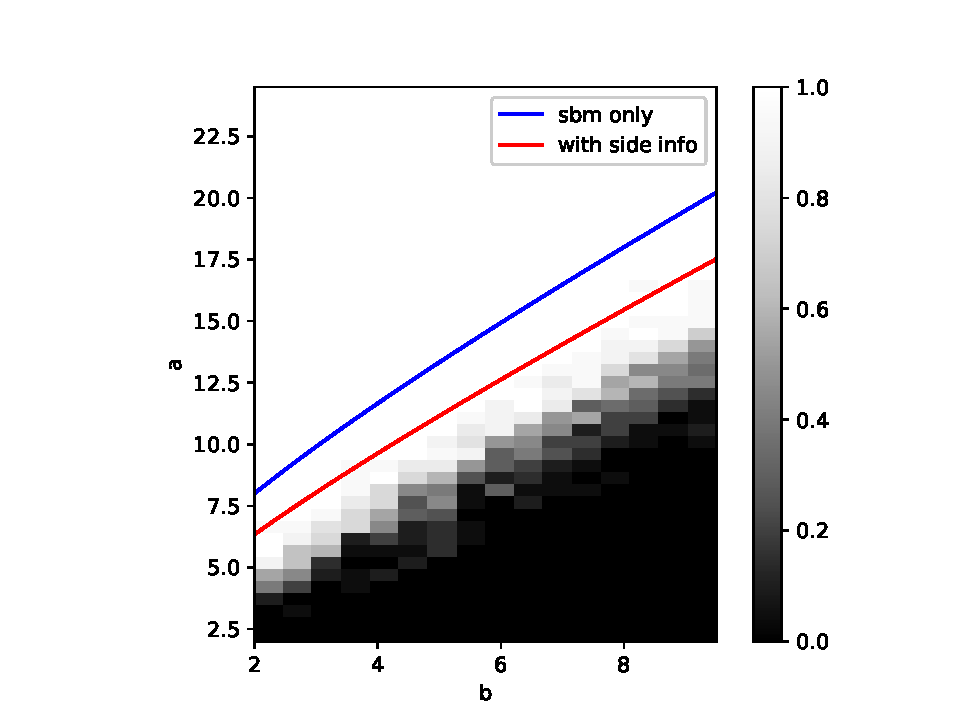
\includegraphics[width=0.8\textwidth]{new_results.pdf}
    \caption{有(无)辅助信息的分界线与SDP算法恢复性能的比较}
    \label{fig:my_label}
\end{figure}

\section{本章小结}\label{sec:summary_sbmsi}
本章研究了带有辅助信息的随机块模型(SBMSI)的精确恢复问题。
具体来说,在给出了 SSBMI 的定义后, 
我们首先针对两社团的情形获得了精确恢复的误差衰减速率。
该结果
表明恢复误差可解耦为由辅助信息的雷尼散度和
随机块模型的参数两部分,
从而可以分别进行优化。
另一方面,为
控制恢复误差在给定的允许范围内,
式\eqref{eq:positive_condition_new}
给出了图节点数量和辅助信息采样数量所需满足的条件。
而关于为获得误差率所做的假设 \eqref{eq:oneC} 是否可以进一步放宽
这一问题有待于进一步研究。

其次,基于半正定规划(SDP)的数学模型
我们还提出了一个实现 SBMSI 精确恢复的算法。
随着图规模的增大,该算法的恢复误差以多项式的速率收敛到零。
能否将SDP恢复算法拓展到多个社团的情形(有辅助信息)目前是一个有
研究价值的开放问题。
